\documentclass{article}

\usepackage[left=2cm,right=2cm, top=2cm, bottom = 2cm]{geometry}
\usepackage{amsfonts}
%%%\usepackage{array}

\usepackage{amsmath}
\usepackage{xcolor}

\usepackage{tikz}
\usepackage{subfigure}

\pagestyle{empty}

\setlength{\tabcolsep}{15pt}
%%%\renewcommand{\arraystretch}{2.5}

%%%\makeatletter
%%%\newcommand{\thickhline}{%
%%%    \noalign {\ifnum 0=`}\fi \hrule height 2pt
%%%    \futurelet \reserved@a \@xhline
%%%}
%%%\newcolumntype{!}{@{\hskip\tabcolsep\vrule width 2pt\hskip\tabcolsep}}
%%%\makeatother

\newcommand{\deriv}[2]{\frac{\mathrm{d}#1}{\mathrm{d}#2}}




\begin{document}

\title{Velocity and Differentiation}
\date{}

\maketitle
\thispagestyle{empty}

\Large

\textbf{\underline{Objective: To have an intuitive understanding of differentiation as}}

\textbf{\underline{it applies to velocity and rates of change.}}



\vspace{5mm}


{\bf Warm-up: Average and Instantaneous Speed:}

\vspace{5mm}

Usain Bolt runs 100m in 10s. 
\begin{enumerate}
	\item What is his average speed?
	\item Suppose the acceleration Bolt achieves is a constant, $a$. It can be shown that the equation of his motion will then be $s=\frac{1}{2}at^2$, where $s$ is distance travelled and $t$ is time. Find $a$.
	\item Find the time after which Bolt has run 50m. Hence find his average speed over the first 50m.
	\item Suppose we want to know how fast Bolt is running after exactly 6s. We can estimate this as follows:
		\begin{enumerate}
			\item Find the distance travelled after 6s.
			\item Find the distance travelled after 7s.
			\item Hence find the average speed between 6s and 7s.
		\end{enumerate}
	\item Now find a more accurate estimate for Bolt's speed at 6s, by using the distance travelled after 6s and after 6.5s.
	\item Now find a more accurate estimate still, by using 6s and 6.1s.
	\item Now we generalise this:
		\begin{enumerate}
			\item Let $h$ be very small. Find the distance Bolt travels between time $t$ and time $t+h$.
			\item Hence find Bolt's average speed between time $t$ and time $t+h$.
			\item What happens to this average speed as we make $h$ smaller and smaller, to make the approximation more accurate?
			\item What therefore is Bolt's instantaneous speed as he crosses the finish line?
		\end{enumerate}
\end{enumerate}



\clearpage


{\bf Theory: Rates of Change:}

\vspace{5mm}

Speed, as seen in the above example, is the rate of change of position with time. Rates of change occur in lots of situations; as well as speed, there is acceleration (rate of change of velocity), electrical current (rate of movement of current), inflation (rate of change of the value of money), road gradient (rate of change of the road height), and countless more. Differentiation is the mathematical study of rates of change.\bigskip


First let's consider the average rate of change over a time interval. This is straightforward to calculate; if $f(t)$ is the quantity we're measuring (which varies with time, so is expressed as a function of time), then the change between $t_1$ and $t_2$ is $f(t_2)-f(t_1)$, and it took time $t_2-t_1$ to make this change. So the average rate of change is
\[\frac{f(t_2)-f(t_1)}{t_2-t_1}.\]


We can visualise this graphically. If we have a graph of $f(t)$ against $t$, then this average rate of change is the gradient of the chord between $(t_1,f(t_1))$ and $(t_2,f(t_2))$. Below is the graph of Usain Bolt's position $s$ against time $t$ from the warm-up, with the average speed of $12\mathrm{ms}^{-1}$ between 4s and 8s shown:

\begin{center}
\begin{tikzpicture}
	\draw[->] (0,0) -- (10,0);
	\draw[->] (0,0) -- (0,10);
	\node[right] at (10,0) {$t$};
	\node[above] at (0,10) {$s$};
	
	\draw[blue, thick, domain=0:10] plot (\x, {\x^2/10});
	
	\draw[red] (4,1.6) -- (8,6.4);
	\draw[dashed] (4,1.6) -- (8,1.6) -- (8,6.4);
	\node[right] at (8,6.4) {$(8,64)$};
	\node[left] at (4,1.6) {$(4,16)$};
	\node[below] at (6,1.6) {$8-4=4\mathrm{s}$};
	\node[right] at (8,4) {$64-16=48\mathrm{m}$};
	\node[above left] at (6,4) {$\frac{48\mathrm{m}}{4\mathrm{s}}=12\mathrm{ms}^{-1}$};
	
	\node[below left] at (0,0) {0};
	\foreach \i in {2,4,6,8,10}{
		\node[below] at (\i,0) {$\i$};
		\node[left] at (0,\i) {$\i 0$};
	}
\end{tikzpicture}
\end{center}



The meaning of this average speed is that Bolt covered the distance from 16m to 64m in the same time as a person running at a constant speed of $12\mathrm{ms}^{-1}$ would have. Average rates of change show how quickly something would have to have changed \textit{at a constant rate} to undergo the same total change in a given amount of time as it actually did with a potentially varying rate.\bigskip


If we want to find the \textit{instantaneous} rate of change of a quantity, it's not even clear what we mean, let alone how to find it. Instead, we find the average rate of change over a very small time interval. We then make this time interval smaller and smaller and look at how the average rate of change behaves as the length of the time interval becomes arbitrarily small. We illustrate this below, taking various values of $h$, smaller each time, and finding Bolt's average speed between 4s and $(4+h)$s.

\begin{figure}
\centering

\subfigure{
	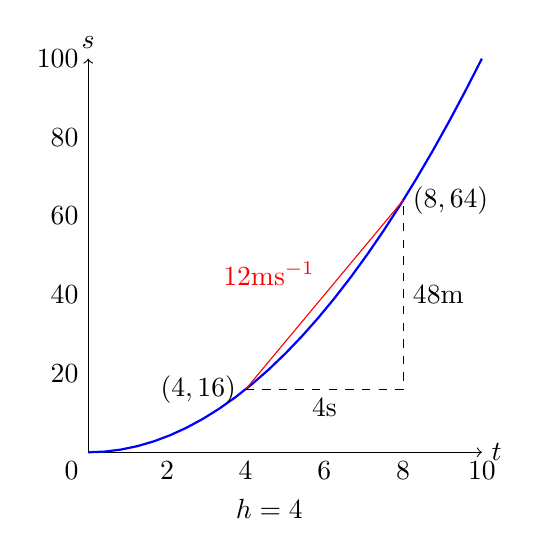
\begin{tikzpicture}[scale=0.5]
		\draw[->] (0,0) -- (10,0);
		\draw[->] (0,0) -- (0,10);
		\node[right] at (10,0) {$t$};
		\node[above] at (0,10) {$s$};
		
		\draw[blue, thick, domain=0:10] plot (\x, {\x^2/10});
		
		\draw[red] (4,1.6) -- (8,6.4);
		\draw[dashed] (4,1.6) -- (8,1.6) -- (8,6.4);
		\node[right] at (8,6.4) {$(8,64)$};
		\node[left] at (4,1.6) {$(4,16)$};
		\node[below] at (6,1.6) {$4\mathrm{s}$};
		\node[right] at (8,4) {$48\mathrm{m}$};
		\node[red,above left] at (6,4) {$12\mathrm{ms}^{-1}$};
		
		\node[below left] at (0,0) {0};
		\foreach \i in {2,4,6,8,10}{
			\node[below] at (\i,0) {$\i$};
			\node[left] at (0,\i) {$\i 0$};
		}
		
		\node[below] at (current bounding box.south) {$h=4$};
	\end{tikzpicture}
}
\subfigure{
	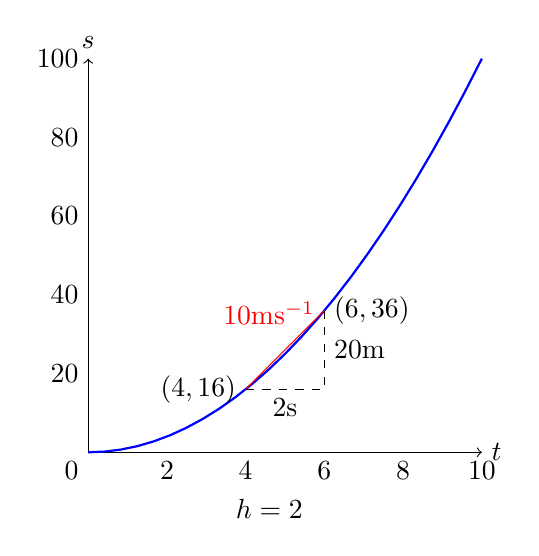
\begin{tikzpicture}[scale=0.5]
		\draw[->] (0,0) -- (10,0);
		\draw[->] (0,0) -- (0,10);
		\node[right] at (10,0) {$t$};
		\node[above] at (0,10) {$s$};
		
		\draw[blue, thick, domain=0:10] plot (\x, {\x^2/10});
		
		\draw[red] (4,1.6) -- (6,3.6);
		\draw[dashed] (4,1.6) -- (6,1.6) -- (6,3.6);
		\node[right] at (6,3.6) {$(6,36)$};
		\node[left] at (4,1.6) {$(4,16)$};
		\node[below] at (5,1.6) {$2\mathrm{s}$};
		\node[right] at (6,2.6) {$20\mathrm{m}$};
		\node[red,above left] at (6,3) {$10\mathrm{ms}^{-1}$};
		
		\node[below left] at (0,0) {0};
		\foreach \i in {2,4,6,8,10}{
			\node[below] at (\i,0) {$\i$};
			\node[left] at (0,\i) {$\i 0$};
		}
		
		\node[below] at (current bounding box.south) {$h=2$};
	\end{tikzpicture}
}
	
\subfigure{
	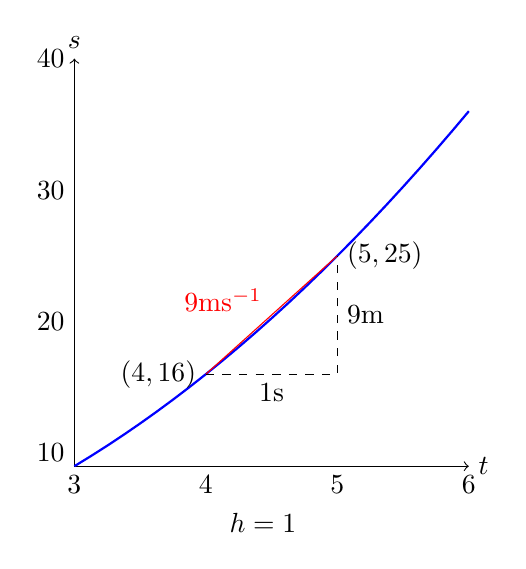
\begin{tikzpicture}[scale=1.67]
		\draw[->] (3,0.9) -- (6,0.9);
		\draw[->] (3,0.9) -- (3,4);
		\node[right] at (6,0.9) {$t$};
		\node[above] at (3,4) {$s$};
		
		\draw[blue,thick,domain=3:6] plot (\x,{\x^2/10});
		
		\draw[red] (4,1.6) -- (5,2.5);
		\draw[dashed] (4,1.6) -- (5,1.6) -- (5,2.5);
		\node[right] at (5,2.5) {$(5,25)$};
		\node[left] at (4,1.6) {$(4,16)$};
		\node[right] at (5, 2.05) {$9\mathrm{m}$};
		\node[below] at (4.5,1.6) {$1\mathrm{s}$};
		\node[red,above left] at (4.5,2) {$9\mathrm{ms}^{-1}$};
		
		
		\foreach \i in {3,4,5,6}{
			\node[below] at (\i,0.9) {$\i$};
		}
		
		\foreach \i in {1,2,3,4}{
			\node[left] at (3,\i) {$\i 0$};
		}
		
		\node[below] at (current bounding box.south) {$h=1$};
	\end{tikzpicture}
}
\subfigure{
	\begin{tikzpicture}[scale=2.5]
		\draw[->] (3,0.9) -- (5,0.9);
		\draw[->] (3,0.9) -- (3,3);
		\node[right] at (5,0.9) {$t$};
		\node[above] at (3,3) {$s$};
		
		\draw[blue,thick,domain=3:5] plot (\x,{\x^2/10});
		
		\draw[red] (4,1.6) -- (4.5,2.025);
		\draw[dashed] (4,1.6) -- (4.5,1.6) -- (4.5,2.025);
		\node[right] at (4.5,2.025) {$(4.5,2.025)$};
		\node[left] at (4,1.6) {$(4,16)$};
		\node[right] at (4.5, 1.8) {$4.025\mathrm{m}$};
		\node[below] at (4.3,1.6) {$0.5\mathrm{s}$};
		\node[red,above left] at (4.3,1.8) {$8.05\mathrm{ms}^{-1}$};
		
		
		\foreach \i in {3,4,5}{
			\node[below] at (\i,0.9) {$\i$};
		}
		
		\foreach \i in {1,2,3,4}{
			\node[left] at (3,\i) {$\i 0$};
		}
		
		\node[below] at (current bounding box.south) {$h=0.5$};
	\end{tikzpicture}
}


\end{figure}





Rather than computing the gradient (average rate of change) for lots of different values of $h$ and seeing what happens as $h$ gets smaller, we can proceed algebraically. The distance travelled between times $t$ and $t+h$ is $(t+h)^2-t^2=t^2+2th+h^2-t^2=2th+h^2$. Dividing this by the difference in time of $t+h-t=h$, we find that Bolt's average speed between $t$ and $t+h$ is
\[\frac{2th+h^2}{h}=2t+h.\]

We can see that as $h$ gets close to 0, this gets close to $2t$. So the instantaneous speed at time $t$ is $2t$.\bigskip

In general, given a function $f(t)$, we find the instantaneous rate of change of $f$ at time $t$ by computing
\[\frac{f(t+h)-f(t)}{h}\]
and studying what happens as $h$ gets very small. We will look at this more carefully on the next sheet.


\clearpage



\textbf{Practice:}

\vspace{5mm}

\begin{enumerate}
	\item Let $f(t)=7t-4$. Find the rate of change of $f$ with respect to $t$.
	\item Let $f(x)=4x^2-3x+1$. Find the rate of change of $f$ with respect to $x$.
	\item The charge $Q$ on one plate of a capacitor varies with time according to $Q=9t-t^3$, where $Q$ is measured in millicoulombs and time in milliseconds. Find the current (in amps---coulombs per second) at time $t$. Find the time at which no current flows. Note: this is probably not an electrically realistic function for charge varying with time!
	\item After going over a speed bump, a car oscillates up and down on its suspension. Suppose its vertical height $y$ obeys the equation $y=\sin(t)$. Find the instantaneous rate of change of height with respect to $t$. You will need the small-angle approximations: when $h$ is very close to 0, $\sin(h)\approx h$ and $\cos(h)\approx 1-\frac{h^2}{2}$; we shall see where these come from next time.
\end{enumerate}





\clearpage


{\bf Key Points to Remember:}

\vspace{5mm}

\begin{enumerate}
\item The average rate of change of a function $f(t)$ between times $t_1$ and $t_2$ is
	\[\frac{f(t_2)-f(t_1)}{t_2-t_1}.\]
\item If we take $h$ small and look at the average rate of change of $f$ between $t$ and $t+h$, we get
	\[\frac{f(t+h)-f(t)}{h}.\]
\item By looking at the behaviour of this quantity as $h$ gets very close to 0, we gain an understanding of the instantaneous rate of change of $f$ at a point.
\end{enumerate}

\bigskip

This was an introduction to the idea behind differentiation; next time, we will give a more detailed account of what differentiation is and how to do it.









\end{document}